\documentclass[12pt,letterpaper]{article}
\usepackage[latin1]{inputenc}
\usepackage[spanish]{babel}
\usepackage{graphicx}
\usepackage[left=2cm,right=2cm,top=2cm,bottom=2cm]{geometry}
\usepackage{graphicx} % figuras
\usepackage{subfigure} % subfiguras
\usepackage{float} % para usar [H]
\usepackage{amsmath}
\usepackage{txfonts}
\usepackage{stackrel} 
\usepackage[latin1]{inputenc}
\usepackage{multirow}
\usepackage{enumerate} % enumerados
\renewcommand{\labelitemi}{$-$}
\renewcommand{\labelitemii}{$\cdot$}
\author{Nelia Escalante}
\title{Caratula}
\begin{document}


\author{Nelia Escalante}
\title{Caratula}

\begin{titlepage}
\begin{center}
\large{UNIVERSIDAD PRIVADA DE TACNA}\\
\vspace*{-0.025in}
\begin{figure}[htb]
\begin{center}

\includegraphics[width=8cm]{./IMG/logo}
\end{center}
\end{figure}
\vspace*{0.15in}
INGENIERIA DE SISTEMAS  \\

\vspace*{0.5in}
\begin{large}
TITULO:\\
\end{large}

\vspace*{0.1in}
\begin{Large}
\textbf{Instalacion de Base de Datos Oracle} \\
\end{Large}

\vspace*{0.3in}
\begin{Large}
\textbf{CURSO:} \\
\end{Large}

\vspace*{0.1in}
\begin{large}
BASE DE DATOS II\\
\end{large}

\vspace*{0.3in}
\begin{Large}
\textbf{DOCENTE:} \\
\end{Large}

\vspace*{0.1in}
\begin{large}
 Ing. Patrick Cuadros Quiroga\\
\end{large}

\vspace*{0.2in}
\vspace*{0.1in}
\begin{large}
Integrantes: \\
\begin{flushleft}
Escalante Maron, Nelia 		\hfill	(2014049551) \\
Salamanca Contreras, Fiorella Rosmery		\hfill	(2015053237) \\
Condori Gutierrez, Flor de Maria            	\hfill	(2015053227) \\
Coaquira Calizaya, Yerson      	\hfill	(2015053225) \\
Espinoza Caso, Lizbeth  		\hfill	(2011040667) \\
\end{flushleft}
\end{large}
\end{center}

\end{titlepage}


 \tableofcontents
 \newpage

 
\section{Introducci\'on} 
En la actual economia impulsada por datos, ningun plan de estudios en ciencias de la computacion o administracion de empresas estaría completo sin un curso sobre bases de datos y administracion de datos. Para poder entender como utilizar los datos que tenemos y encontrar mejores y más innovadoras maneras de administrarlos y utilizarlos, es esencial que entendamos la manera en que las computadoras organizan, utilizan y procesan los datos.

Durante más de 40 aos, Oracle ha estado ayudando a empresas, gobiernos y organizaciones a recopilar, organizar, administrar y utilizar sus datos para mejorar no solo sus negocios, sino también el mundo. 
Oracle la primera Base de Datos Disenada para Grid Computing. es un sistema de gestion de  base de datos relacional fabricado por Oracle Corporation.

Oracle es basicamente una harramienta Cliente/Servidor para la gestion de base de datos la gran potencia que tiene y su elevado precio hace que solo se vea en empresas muy grandes y multinacionales, por norma general. \\
Oracle Corporation: Es una de las mayores companias de software del mundo.Sus producto van desde bases de datos (Oracle) hasta sistemas de gestion, cuanta ademas con herramientas propias de desarrollo para realizar potentes aplicaciones, como Oracle. 
\begin{center}
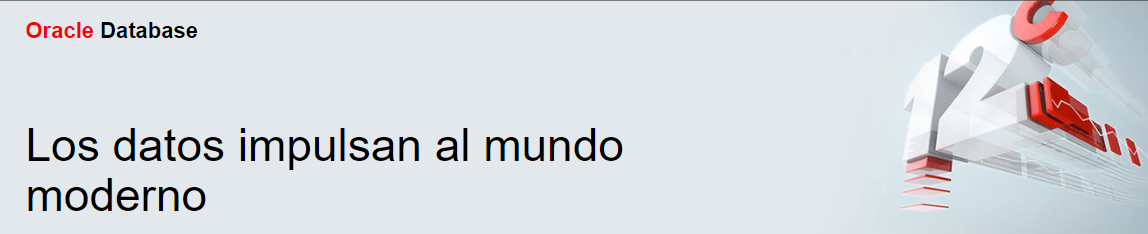
\includegraphics[width=15cm]{IMG/img001.png} 
\end{center}

 \newpage
\section{Objetivos} 
- Realizar la instalacion,  del gestor de base de datos Oracle.

- Especificar las diferentes aplicaciones dentro del lugar de trabajo.

- Determinar los usuarios relacionados para el intercambio de informacion por medio de las aplicaciones de comunicacion.

- Conocer el adecuado funcionamiento de almacenamiento y transmision de datos que permiten ciertas aplicaciones.
\newpage
\section{Oracle Linux modo Terminal (Consola)}
\subsection{Instalacion}
Para poder realizar la instalacion de la base de datos  debemos de tener  el Sistema operativo Oracle Linux. \\
\\Una vez obtenida el Sistema Operativo:\\ 
\\
- Iniciaremos sesion en Oracle Linux. \\
- Usuario OracleServidor  \\
\begin{center}
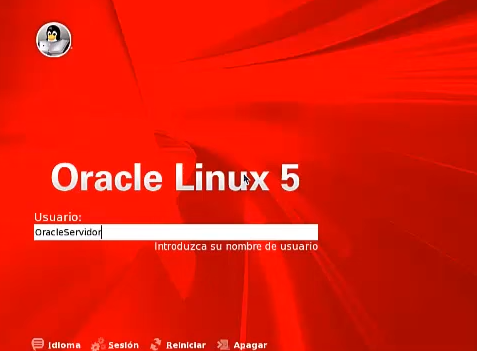
\includegraphics[width=11cm]{IMG/oracle1.png} 
\end{center}
- Ingresamos la contrasena \\
\begin{center}
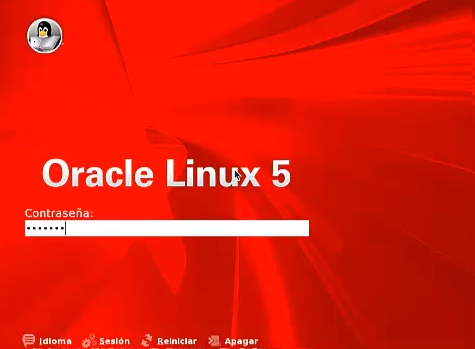
\includegraphics[width=11cm]{IMG/oracle2.png} 
\end{center}
- Enseguida abriremos el terminal en oracle, damos clic derecho y escogemos la opcion de "Abrir Terminal" \\

\begin{center}
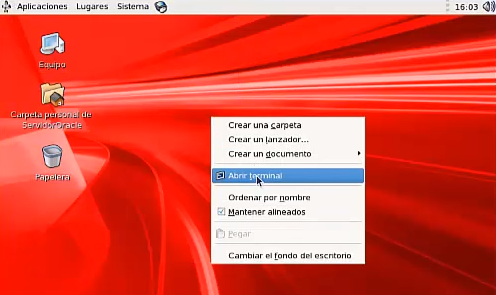
\includegraphics[width=12cm]{IMG/oracle3.png} 
\end{center}

Paso 1: Una vez iniciado sesion con el usuario root abrimos una terminal ejecutamos el comando, lo que va hacer este comando es instalar repositorios que son necesarios para la instalacion de oracle database, veremos que se instalaran con ayuda del internet, esperamos a que se instale, esta accion lo realizamos con el comando. 
\begin{center}

\includegraphics[width=8cm]{./oraclelinux/Comando.png}
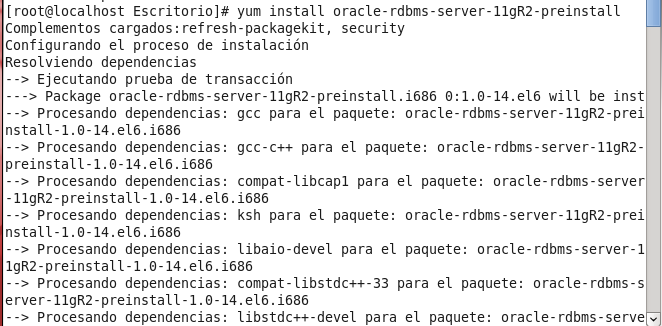
\includegraphics[width=15cm]{./oraclelinux/1.png}
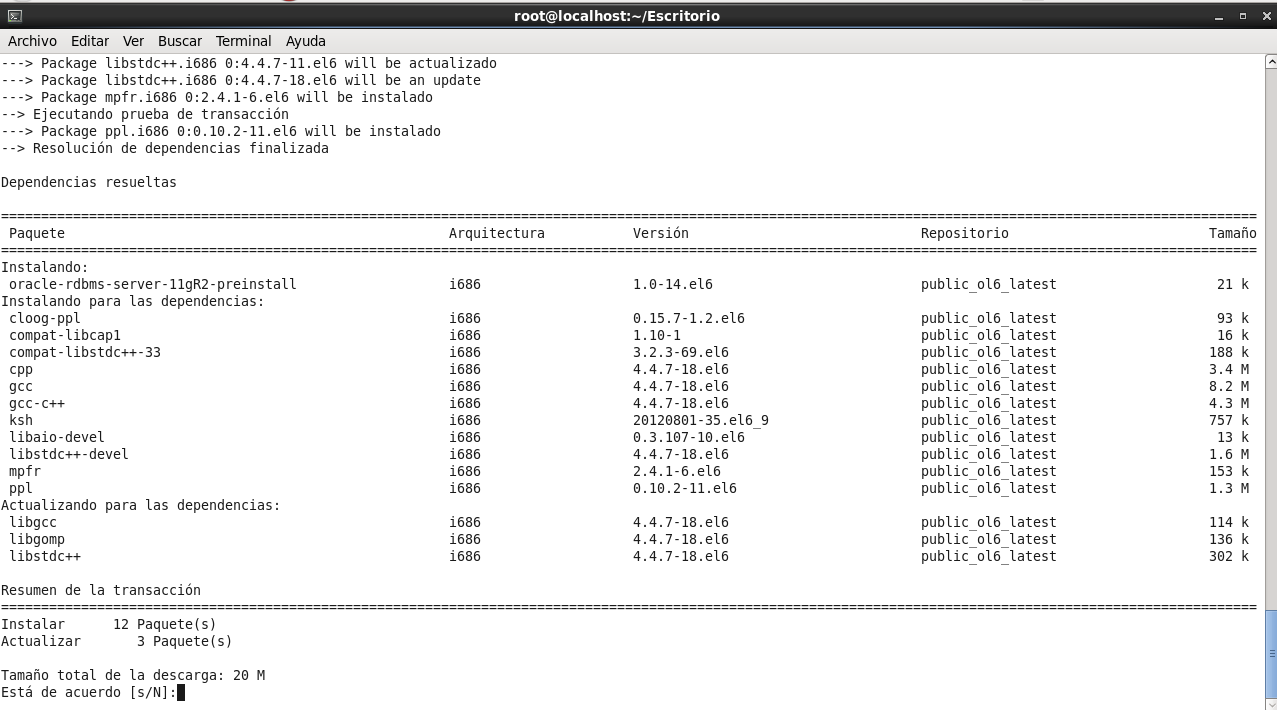
\includegraphics[width=15cm]{./oraclelinux/2.png}
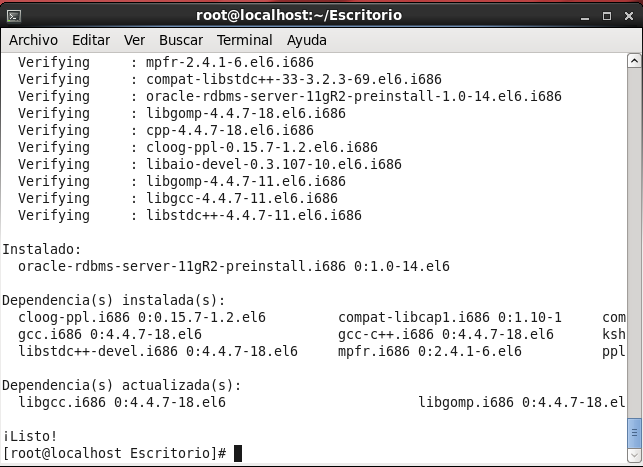
\includegraphics[width=15cm]{./oraclelinux/3.png}
\end{center}

Paso 2 : Una vez instalada todos los repositorios faltantes Creamos la carpeta donde se instalara los db de oracle

\begin{center}
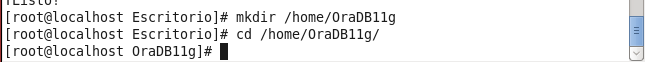
\includegraphics[width=15cm]{./oraclelinux/4.png}
\end{center}
Paso 3 : Montamos un usb con el instalador en este caso tenemos el instaldor en dos partes en archivos zip,una vez montado el usb copiamos los archivos a la carpeta creada anteriormente /home/OraDB11g.

\begin{center}
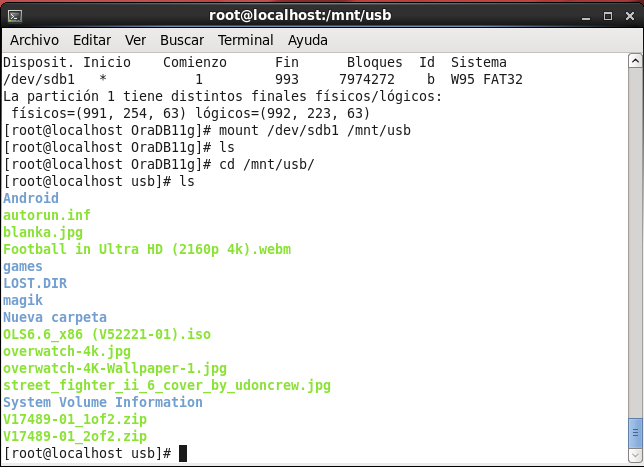
\includegraphics[width=15cm]{./oraclelinux/5.png}
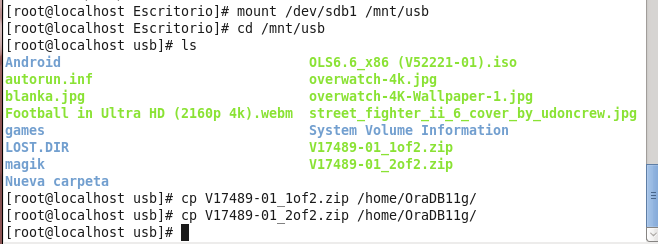
\includegraphics[width=15cm]{./oraclelinux/6.png}
\end{center}

Paso 4 : Una vez copiado los archivos nos dirigimos a la carpeta /home/OraDB11g  para extraer el instalador
\begin{center}
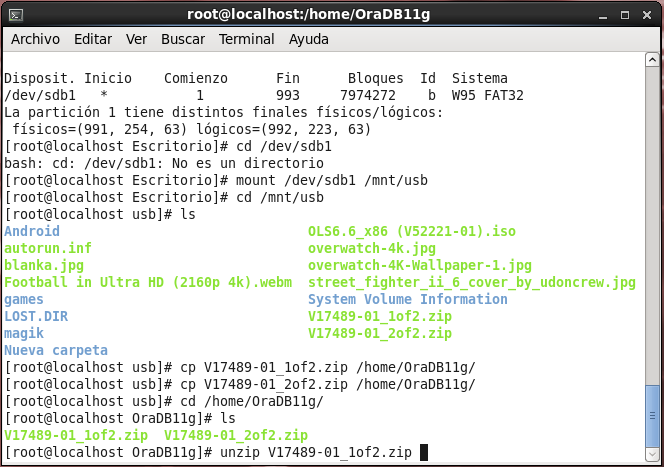
\includegraphics[width=15cm]{./oraclelinux/7.png}
\end{center}
Paso 5 : Una vez extraida se creara un carpeta database.

\begin{center}
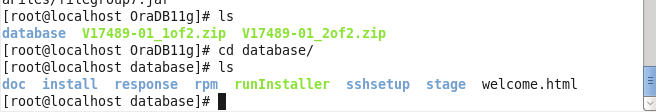
\includegraphics[width=15cm]{./oraclelinux/8.png}
\end{center}
Paso 6 : Ahora para ejecutar el runInstaller debemos iniciar sesion con el usuario oracle para eso de asiganamos una contrasena con el comando passwd.
\begin{center}
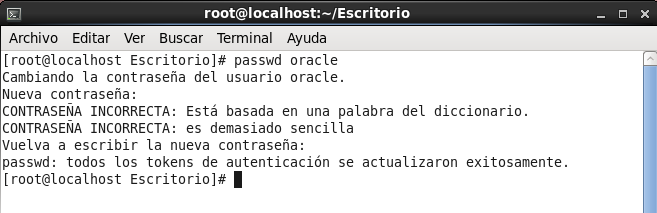
\includegraphics[width=15cm]{./oraclelinux/9.png}
\end{center}

Paso 7 : Luego iniciamos sesion y nos dirimos a la carpeta donde se encuentra el instalador y ejecutamos runInstaller.

\begin{center}
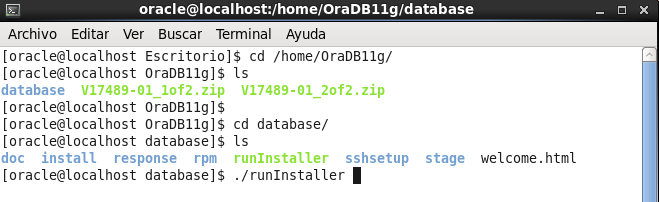
\includegraphics[width=15cm]{./oraclelinux/10.png}
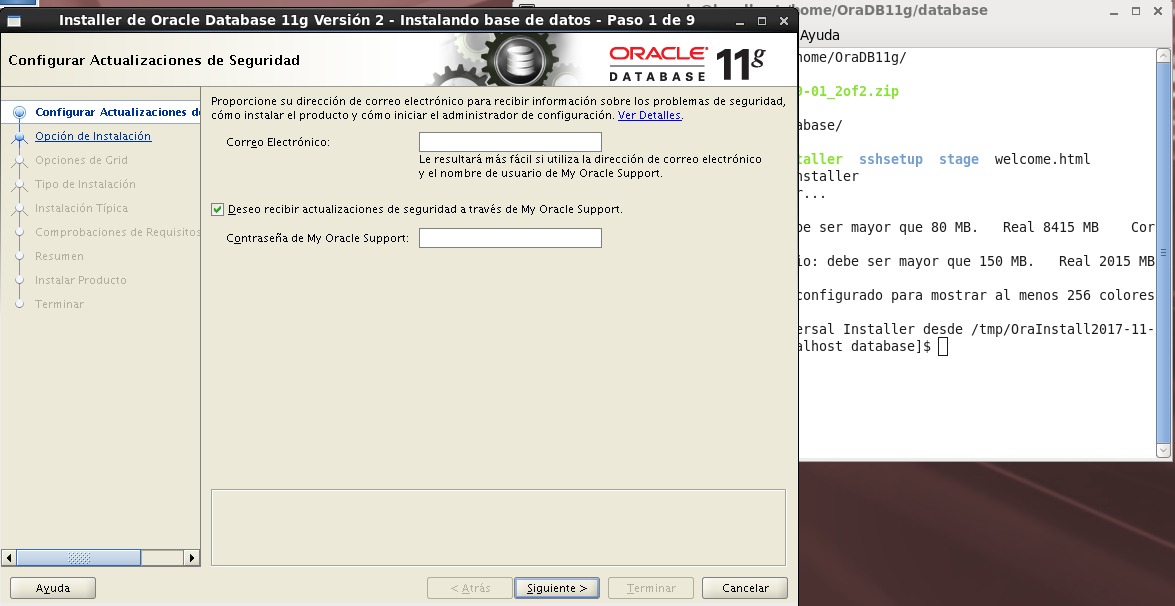
\includegraphics[width=15cm]{./oraclelinux/11.png}\\
Proporcionamos una direccion de correo electronico para recibir informacion sobre los problemas de seguridad.\\
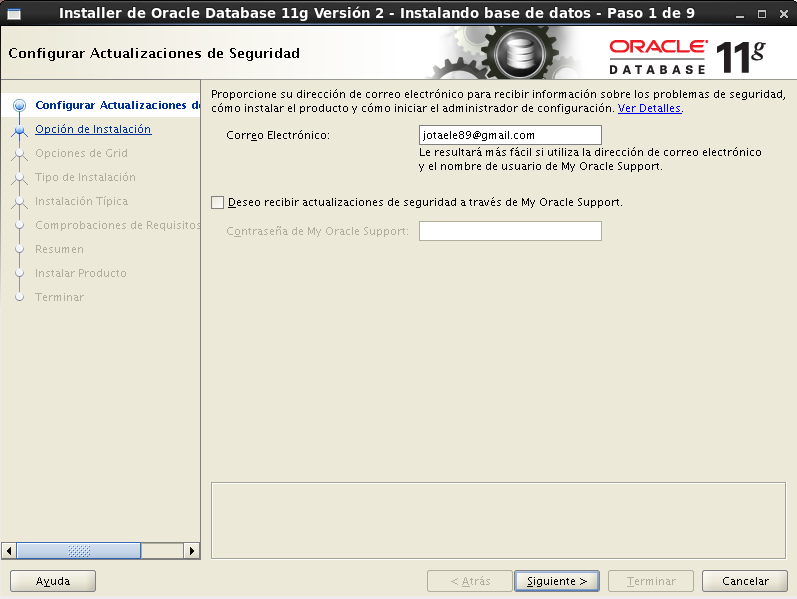
\includegraphics[width=15cm]{./oraclelinux/12.png}\\
Seleccionamos cualquiera de las opciones.\\
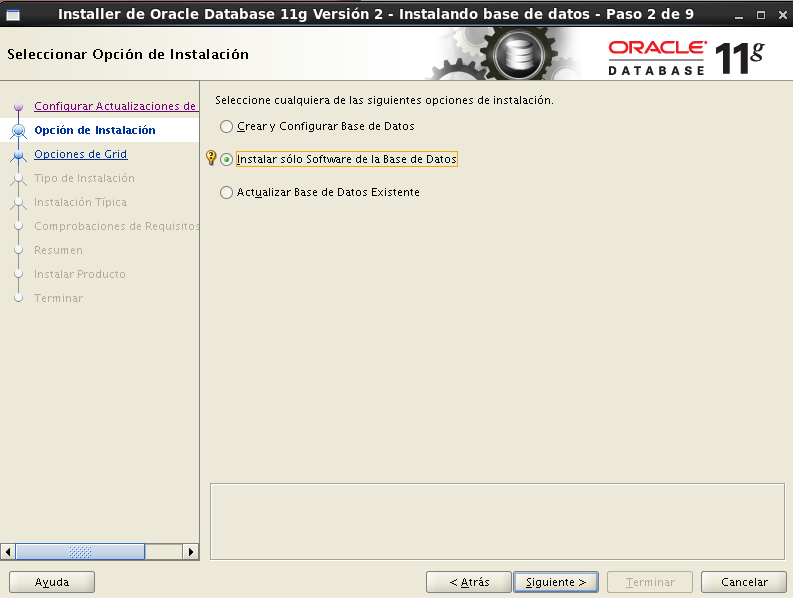
\includegraphics[width=15cm]{./oraclelinux/13.png}\\
Seleccionamos el tipo de instalacion de base de datos.\\
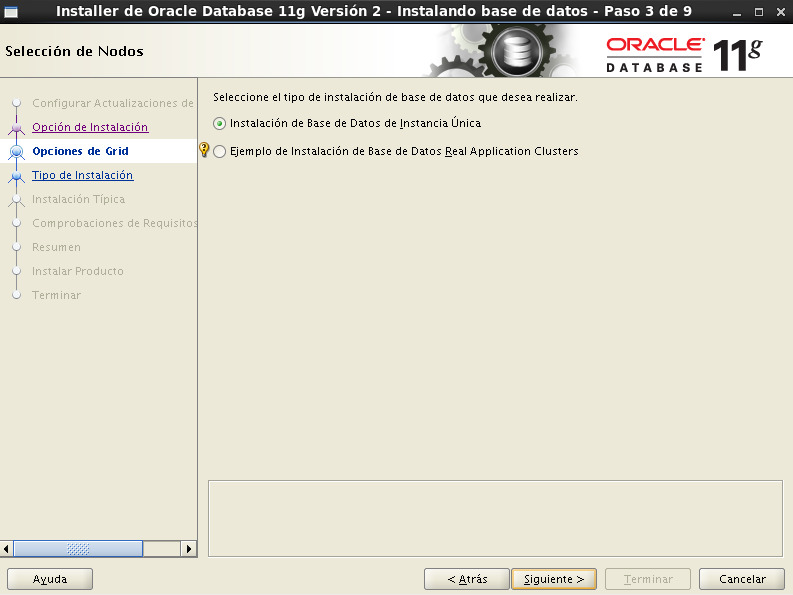
\includegraphics[width=15cm]{./oraclelinux/14.png}\\
Seleccionamos los idiomas en que se ejecutara el producto.\\
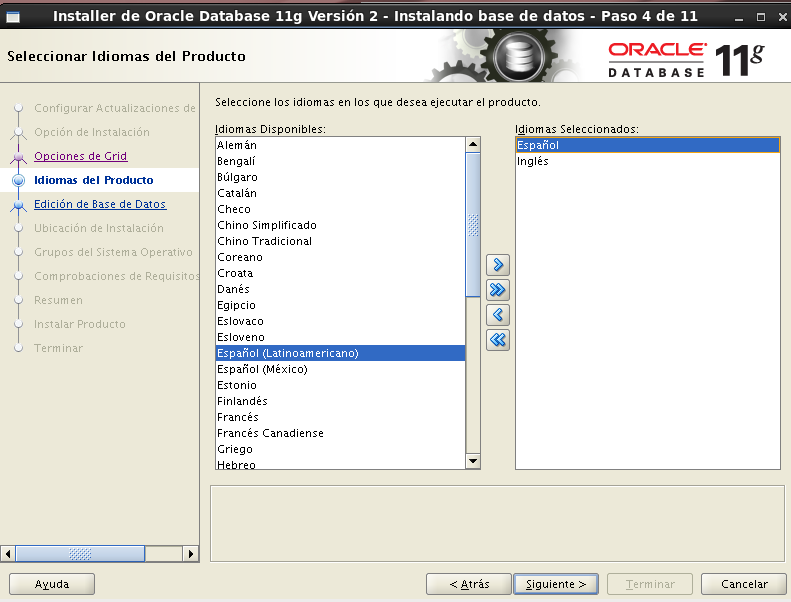
\includegraphics[width=15cm]{./oraclelinux/15.png}\\
Seleccionamos la edicion de base de datos que deseamos instalar.\\
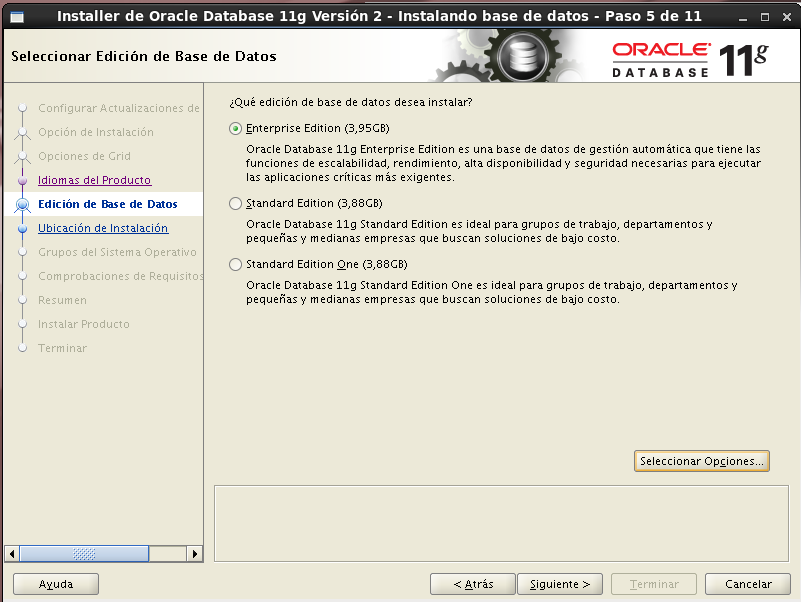
\includegraphics[width=15cm]{./oraclelinux/16.png}\\
Especificamos la ruta de acceso al direcctorio a la base de Oracle.\\
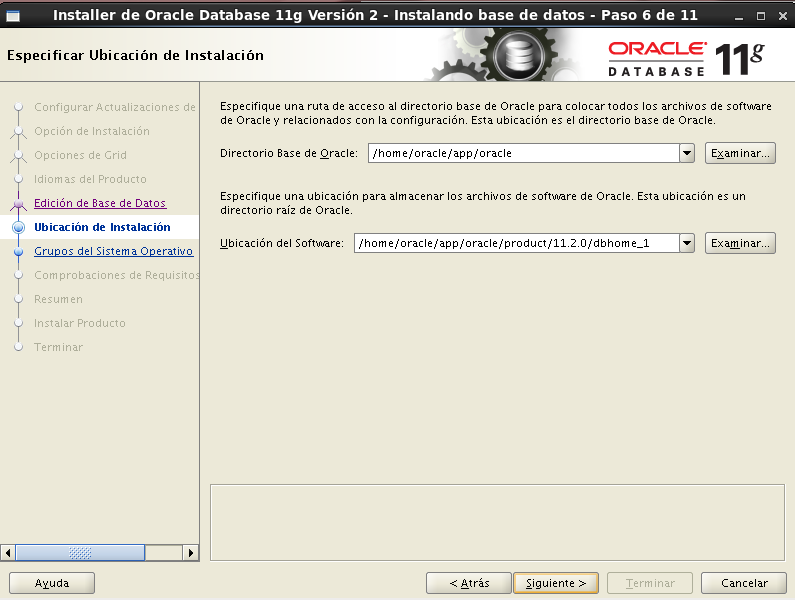
\includegraphics[width=15cm]{./oraclelinux/17.png}\\
Especificamos un directorio para los archivos de instalacion.\\
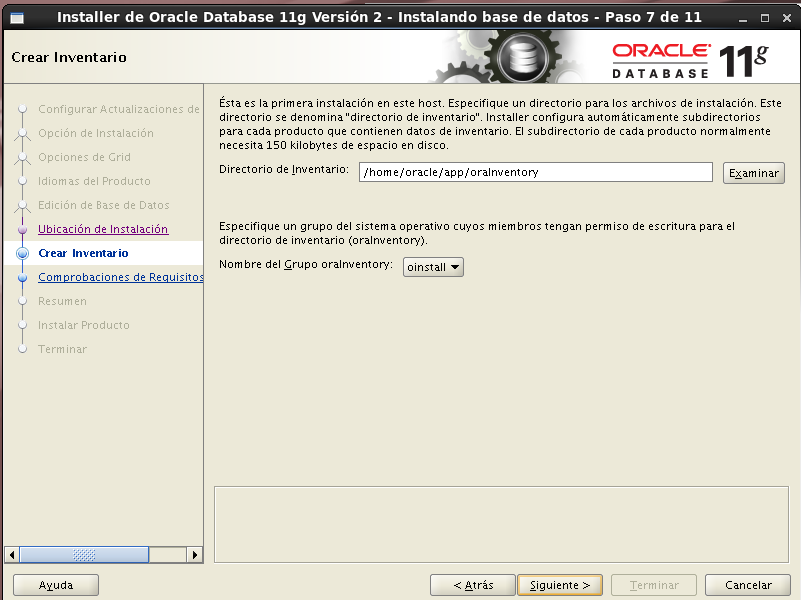
\includegraphics[width=15cm]{./oraclelinux/18.png}\\
Otorgamos los permisos necesarios.\\
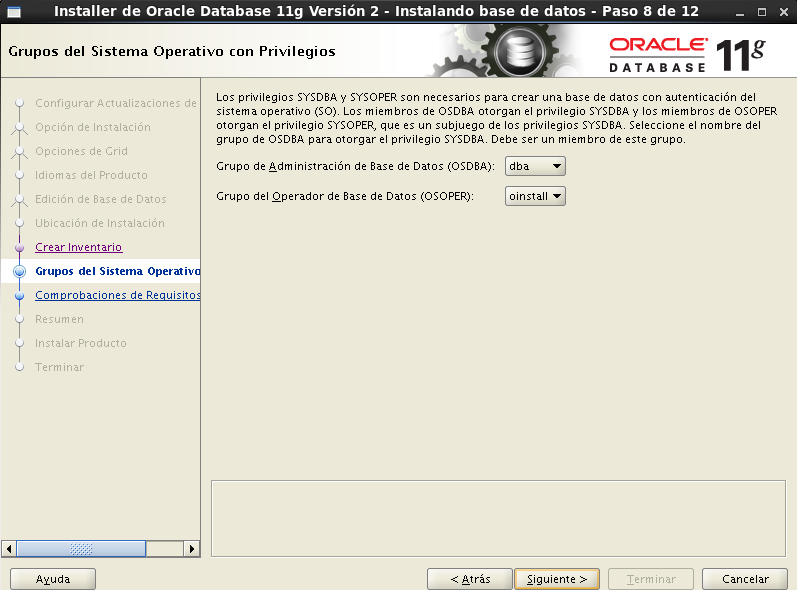
\includegraphics[width=15cm]{./oraclelinux/19.png}\\
Verificara los requisitos minimos de instalacion y configuracion.\\
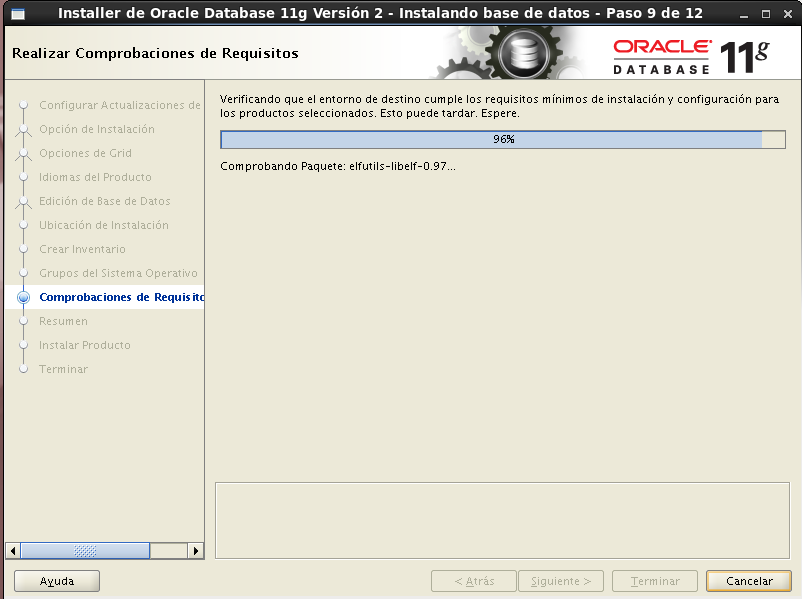
\includegraphics[width=15cm]{./oraclelinux/20.png}\\
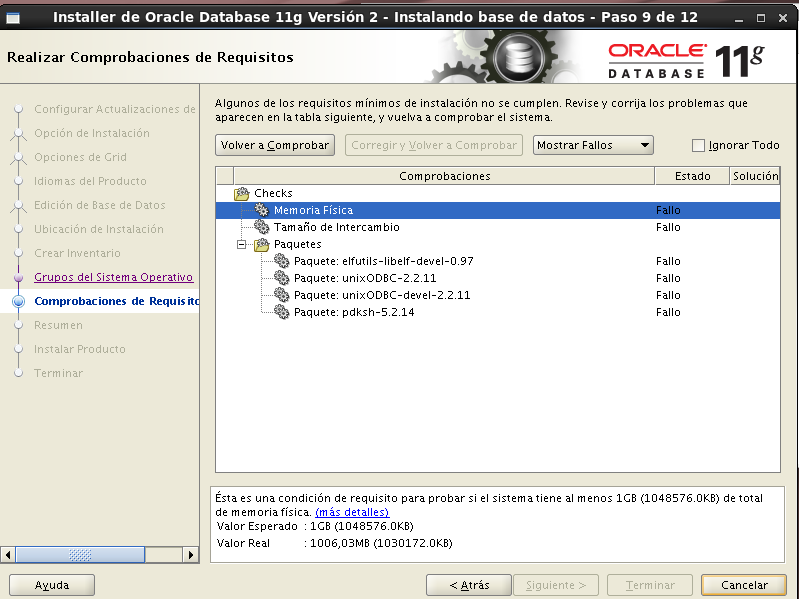
\includegraphics[width=15cm]{./oraclelinux/21.png}\\
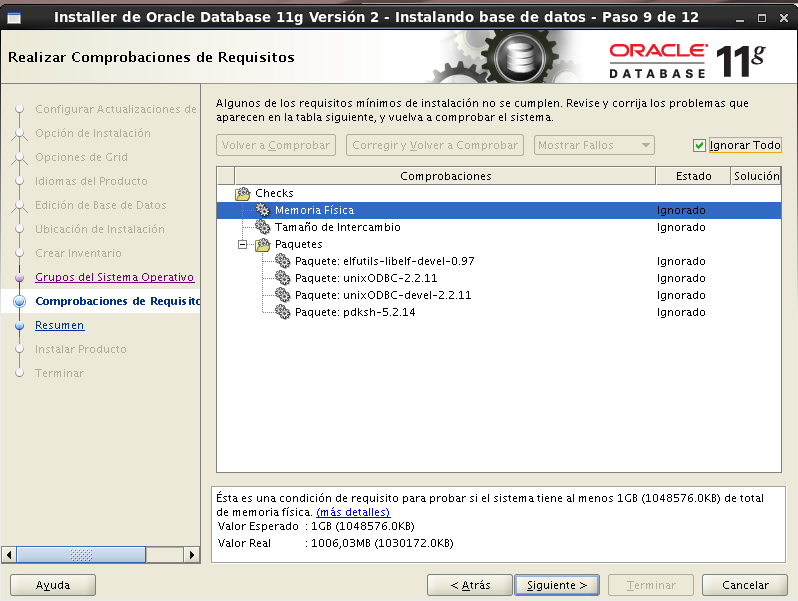
\includegraphics[width=15cm]{./oraclelinux/22.png}\\
Nos mostrara el resumen de lo que vamos a instalar.\\
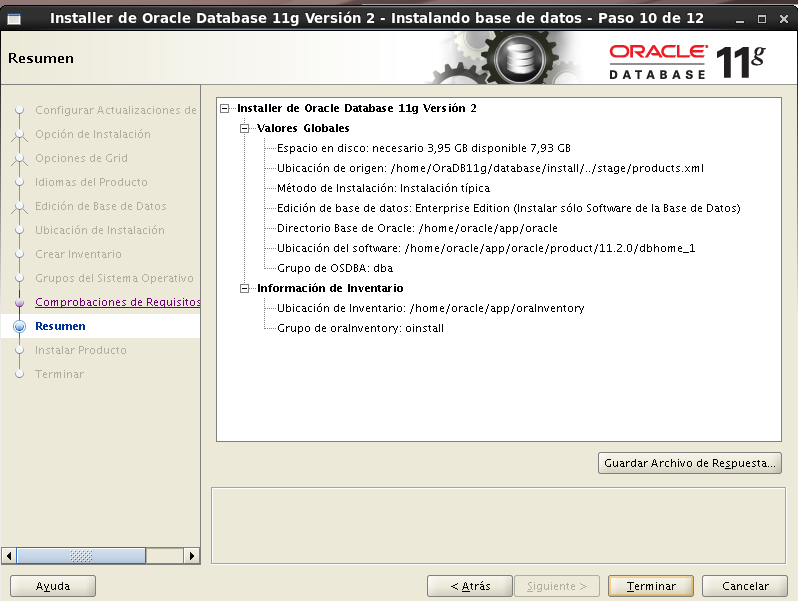
\includegraphics[width=15cm]{./oraclelinux/23.png}\\
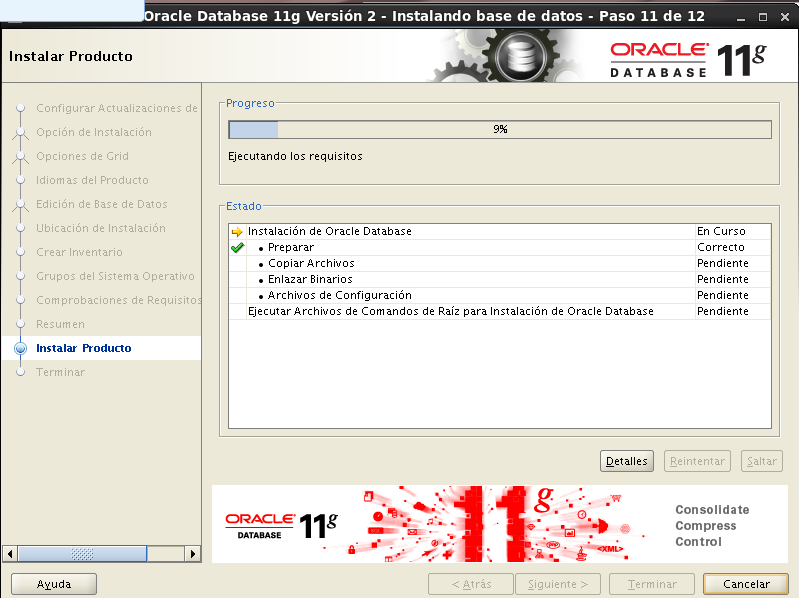
\includegraphics[width=15cm]{./oraclelinux/24.png}\\
Antes de terminar la instalacion nos saltara un ventana donde nos indica que antes de terminar la instalacion debemos ejecutar algunos scripts\\
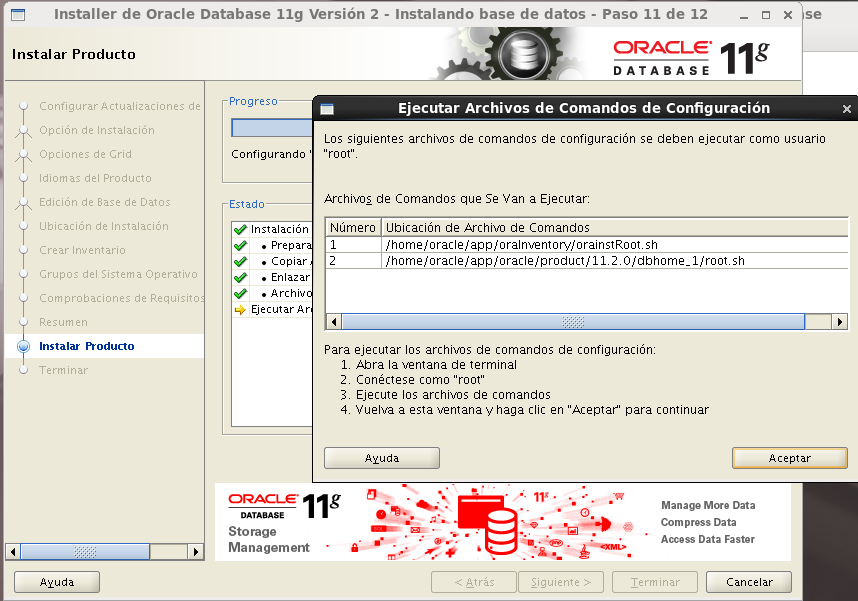
\includegraphics[width=15cm]{./oraclelinux/25.png}\\
Abrimos otra terminal e iniciamos sesion con el usuario "root" y ejecutamos el primer script
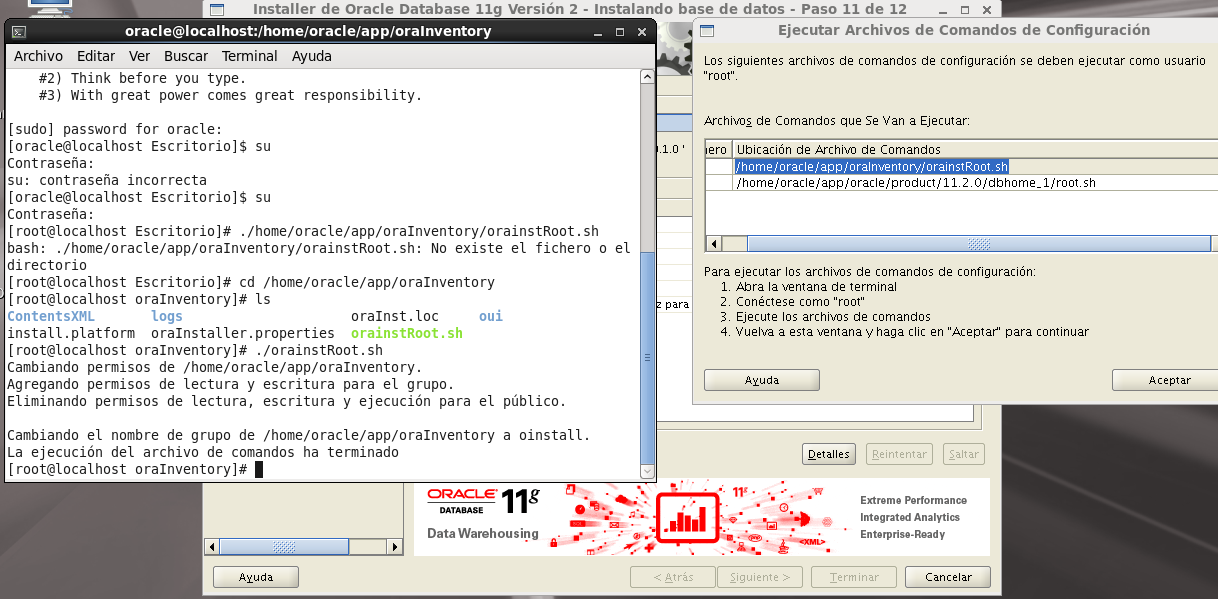
\includegraphics[width=15cm]{./oraclelinux/27.png}\\
Ahora vamos con el segundo  con esto bastara y terminara la instalacion\\
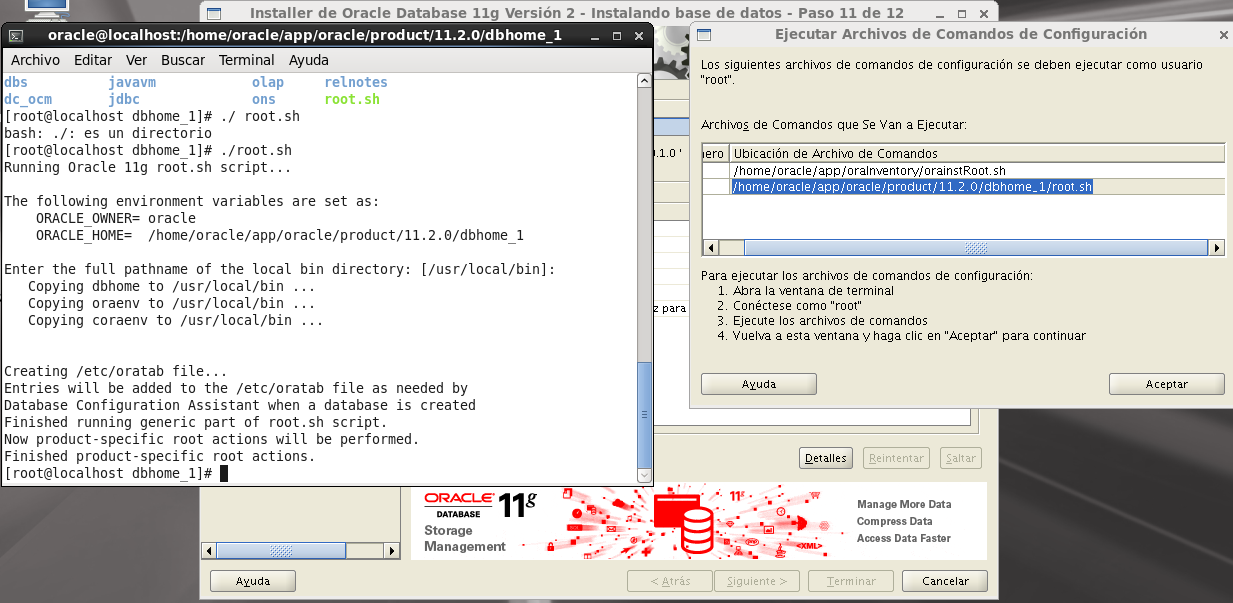
\includegraphics[width=15cm]{./oraclelinux/28.png}\\
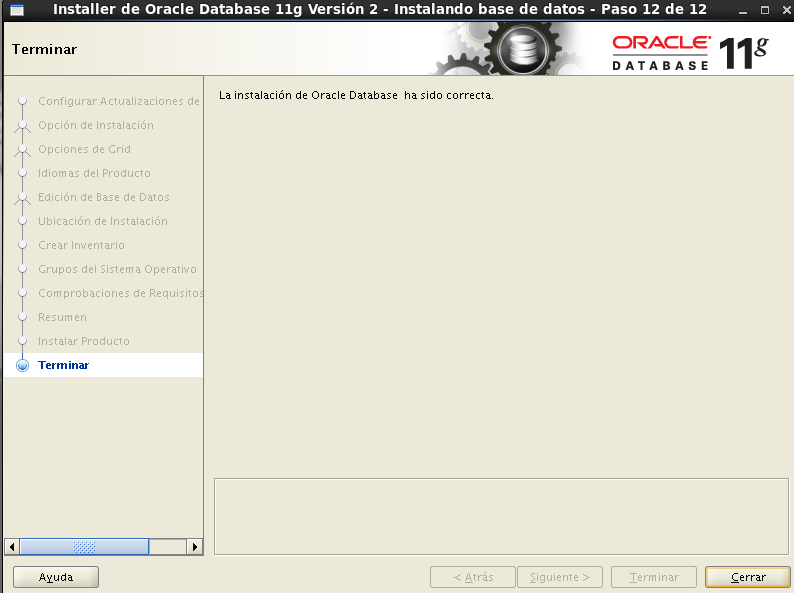
\includegraphics[width=15cm]{./oraclelinux/29.png}\\
\end{center}


\subsection{Configuraci\'on}
Abriremos el sistema de configuraci�n con el comando dbca \\
\begin{center}
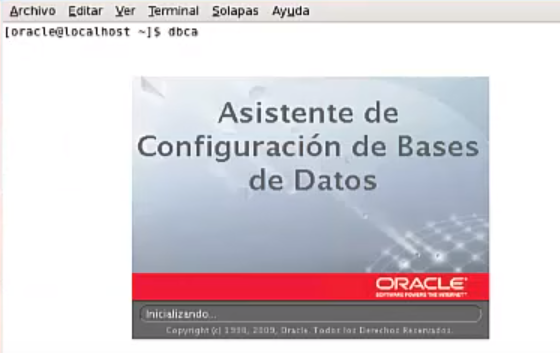
\includegraphics[width=15cm]{oraclelinux/30.png} 
\end{center}
Daremos clic en siguiente. \\
\begin{center}
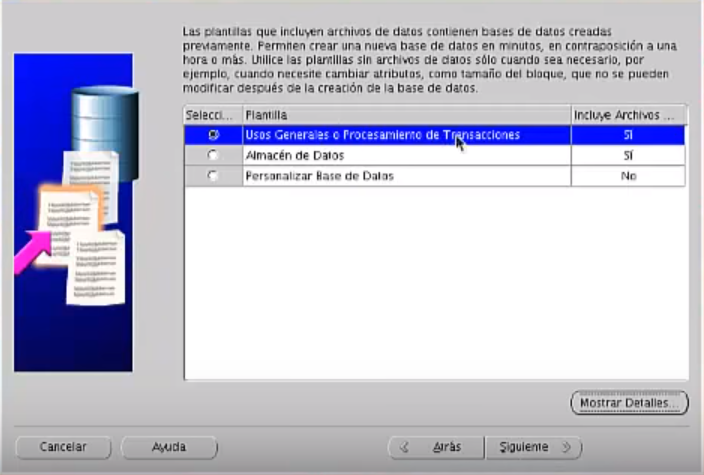
\includegraphics[width=15cm]{oraclelinux/31.png}
\end{center}
A continuaci�n colocaremos el nombre de la base de datos en este caso  prueba. \\
\begin{center}
Ahora esta pidiendo un asistente de configuraci�n de base de datos que es el listener.\\
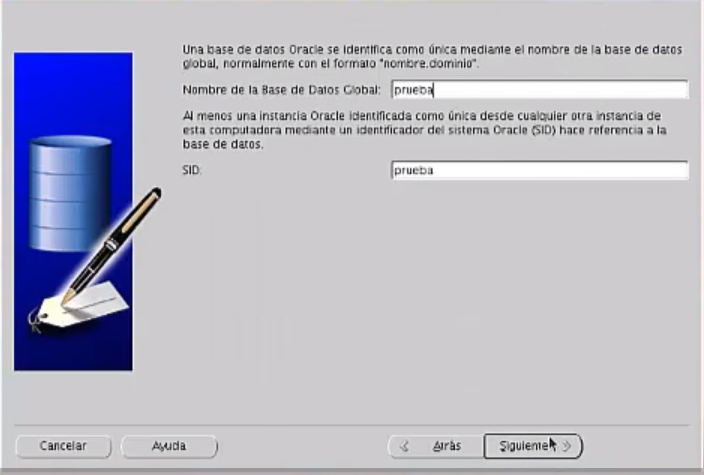
\includegraphics[width=15cm]{oraclelinux/32.png}
\end{center}
Mediante la consola abriremos con el comando netca el asistente de configuraci�n.\\
\begin{center}
	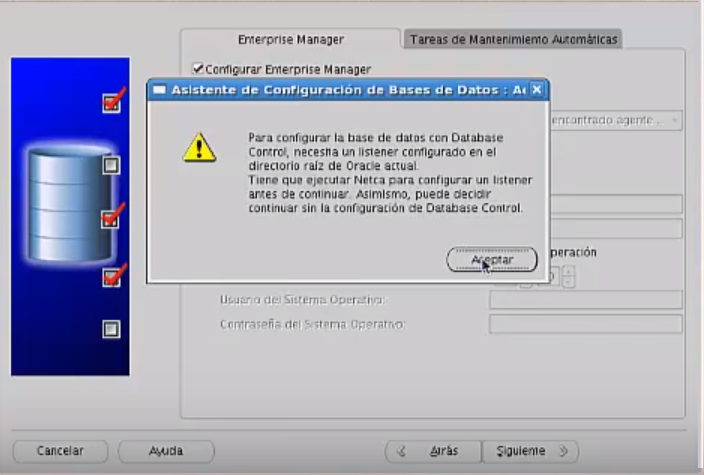
\includegraphics[width=15cm]{oraclelinux/33.png}
\end{center}
Ahora seleccionamos en donde dice configuraci�n de listener daremos clic en siguiente. \\
\begin{center}
	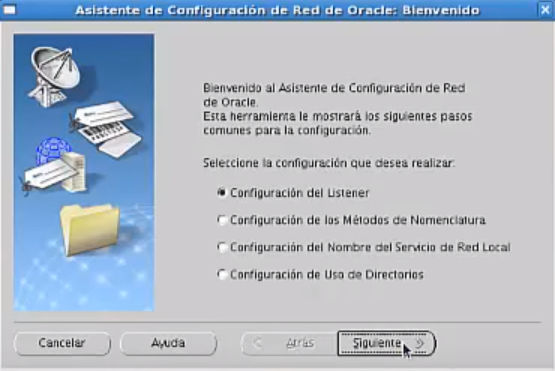
\includegraphics[width=15cm]{oraclelinux/34.png}
\end{center}
\newpage
Digitamos un nombre que sera LISTENER \\
\begin{center}
	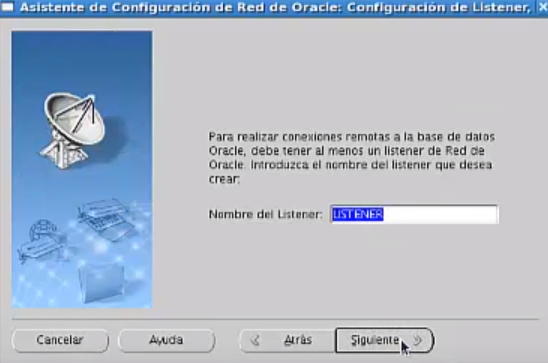
\includegraphics[width=15cm]{oraclelinux/36.png}
\end{center}
Solo daremos clic en siguiente. \\
\begin{center}
	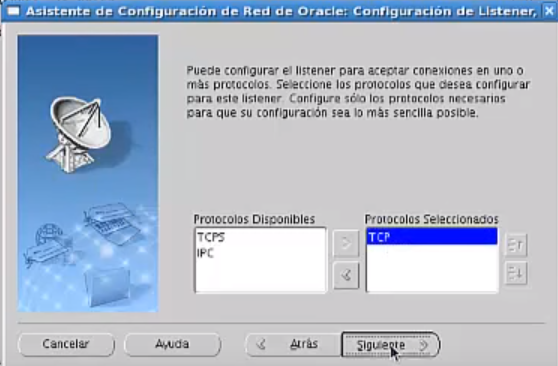
\includegraphics[width=15cm]{oraclelinux/37.png}
\end{center}
\newpage
Seleccionamos usar el numero de puerto.
\begin{center}
	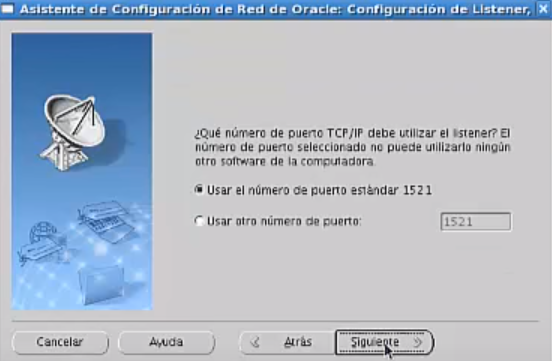
\includegraphics[width=15cm]{oraclelinux/38.png}
\end{center}
Configuraci�n de listener finalizada.
\begin{center}
	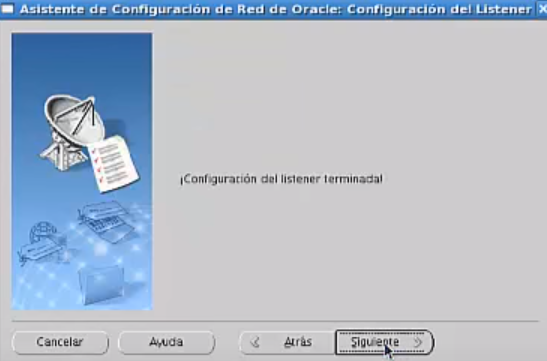
\includegraphics[width=15cm]{oraclelinux/39.png}
\end{center}
\newpage
Colocaremos una contrase�a \\

\begin{center}
	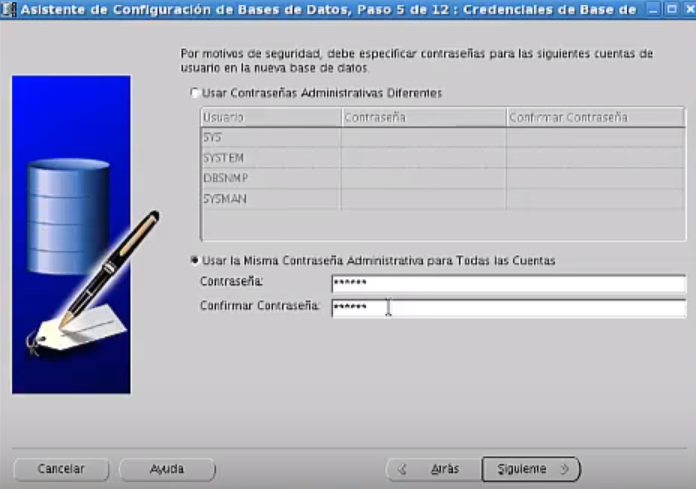
\includegraphics[width=15cm]{oraclelinux/40.png}
\end{center}

clic en siguiente \\
\begin{center}
	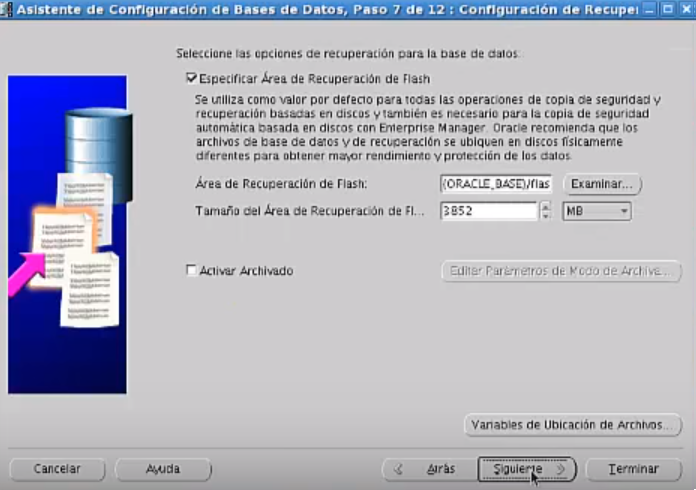
\includegraphics[width=15cm]{oraclelinux/41.png}
\end{center}
\begin{center}
	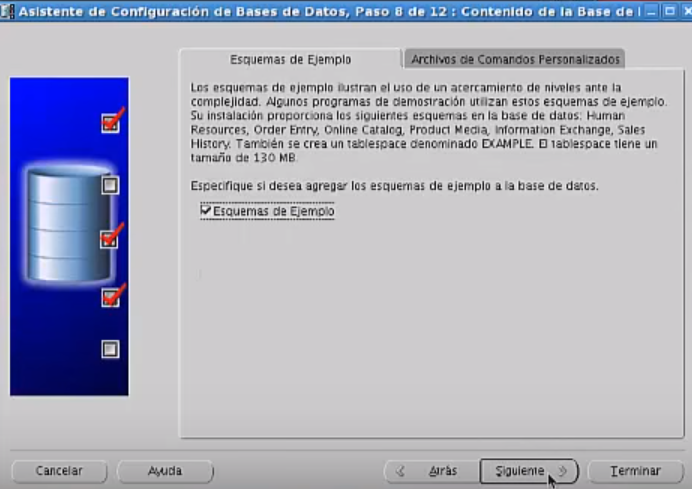
\includegraphics[width=15cm]{oraclelinux/42.png}
\end{center}
\begin{center}
	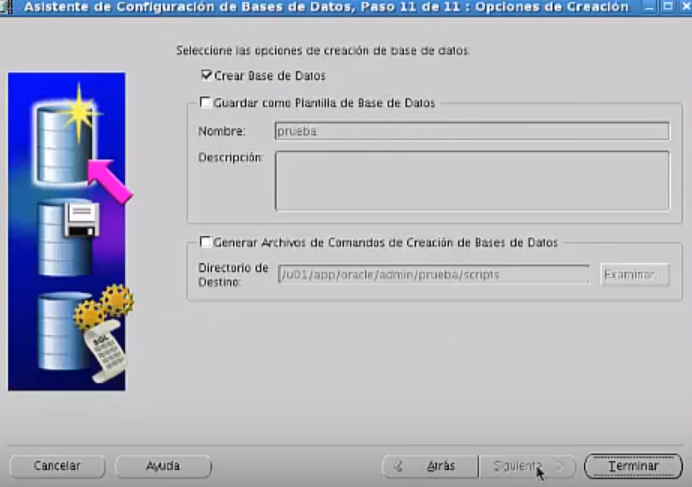
\includegraphics[width=15cm]{oraclelinux/43.png}
\end{center}
\newpage
Se esta creando la base de datos \\
\begin{center}
	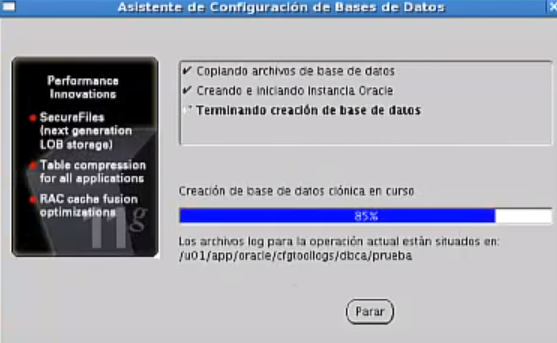
\includegraphics[width=15cm]{oraclelinux/44.png}
\end{center}
visualizamos la conexi�n a sql.
\begin{center}
	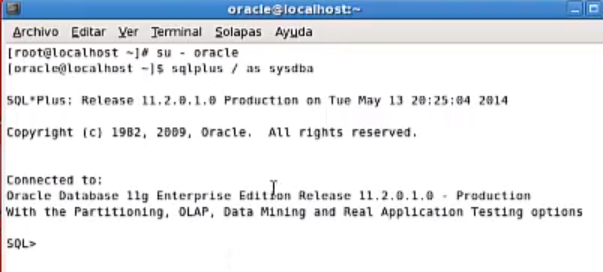
\includegraphics[width=15cm]{oraclelinux/46.png}
\end{center}

\newpage

\section{Windows Server}
\subsection{Instalacio\'on}
Primero descargar el fichero ejecutable desde la p\'agina principal de Oracle.
Despu\'es de descargar el fichero, descomprimir la carpeta que lo contiene,
posteriormente, ubicar el archivo en donde se encuentra el ejecutable y
hacer doble clic en el setup.
\begin{center}
	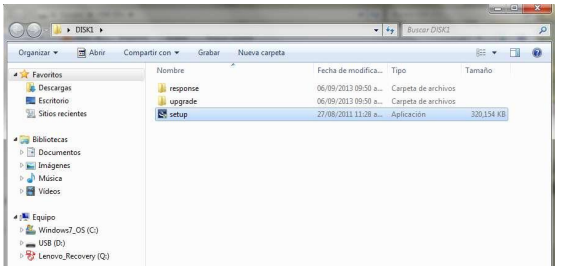
\includegraphics[width=15cm]{./IMG/img1}
\end{center} 
Posteriormente ejecutar esta aplicaci�n y aceptar los permisos aparecer� el
instalador del gestor de base de datos.
\begin{center}
	\includegraphics[width=15cm]{./IMG/img2}
\end{center} 
\newpage
Ahora procedemos a instalarlo y el asistente empezar\'a dicho proceso
\begin{center}
	\includegraphics[width=15cm]{./IMG/img3}
\end{center} 

A continuaci�n nos pedir� el nombre de usuario y una contrase�a, estas deber\'an
ser ingresadas por el Administrador de la base de datos, con esto ingresaremos al
Sistema Gestor de Base de Datos. Finalmente cuando el asistente finaliza con la
instalaci�n iniciaremos la base de datos:\\
Para esto deber\'a ir al men\'u inicio de Windows, clic en todos los programas,
localiza Oracle Database 11g Express Edition y despu\'es en Get Sarted.

\end{document}
